%\documentclass[10pt,preprint]{aastex}
\documentclass[apj]{emulateapj}
\usepackage{txfonts}
\usepackage{graphicx}
\usepackage{natbib}

\newcommand{\kms}{${\rm km \; s^{-1}}$}

\shorttitle{Local Number Density Environments of Massive Galaxies}
\shortauthors{Lifset}

\begin{document} 
\title{Local Number Density Environments of Massive Galaxies}

\author{Noah Lifset\altaffilmark{1}, 3D-HST}
\altaffiltext{1}{Yale University, 260 Whitney Ave., New Haven, CT 06511}

\begin{abstract}

We study the local galaxynumber density environments of very massive galaxies. We select galaxies with mass greater than 10 \textsuperscript{11} solar masses and with a redshift between 0.5 and 2.5. Using both the Nth nearest and aperture radius calculations for local galaxy number density, we are able to study both the immediate environment and general environment. \citet{TOMER}
\end{abstract}
\keywords{Galaxy Number Density}

\section{Introduction}

lots and lots and lots and lots andlots and lots andlots and lots andlots and lots andlots and lots andlots and lots andlots and lots andlots and lots andlots and lots andlots and lots andlots and lots andlots and lots andlots and lots andlots and lots andlots and lots andlots and lots andlots and lots andlots and lots andlots and lots andlots and lots andlots of text.

\section{Sample Selection}

We use 3d hst. We cut off lmass at 9,415 and above because of the completeness from Tal (2014). Talk about edging, even though it only applies to the nth nearest neighbor calculation. 

\section{Data and Analysis}

We use two different methods for calculating local galaxy number density. The first, the nth nearest neighbor calculation, has been shown to be more accurate for immediate environments Cooper (2014). The second, counts in aperture radius, is more accurate for larger and more general environments Cooper (2014).

\subsection{Nth Nearest Calculation}

One of the most common ways of measuring local galaxy number density is using the distance to the nth nearest spectroscopically observed galaxy. Redshift information is used to restrict the pool of neighbors that can be selected from to a given velocity interval. This is done to avoid background and foreground sources. A redshift difference of 0.08 is used here to try and maintain completeness as best as possible. This cut off was selected based on suggestions by Cooper (2014), Tal (2012), and Muldrew (2012). Thus the pool of galaxies that the nth nearest neighbor is being selected from is a cylinder, rather than a sphere. The nth nearest neighbor distance is expressed as a projected surface density $\Sigma$ $_{n}$. The calculation for the projected surface density is $\Sigma$$_{n}$ = n / ($\pi$ R$_{n}$$^{2}$) where R$_{n}$ is the distance to the nth nearest neighbor. 



\subsection{Counts in Aperture Radius Calculation}

Another method for measuring local galaxy number density is counting the number of galaxies within a certain aperture radius. This method once again requires a redshift cut of 0.08. The pool of galaxies counted is then also a cylinder rather than a sphere. The calculation for galaxy number density is simply $\Sigma$$_{r}$ = n$_{gal}$ / ($\pi$ r$^{2}$) where r is the selected aperture radius and n$_{gal}$ is the number of galaxies within that radius.

INCLUDE APERTURE RADIUS COMPARE GRAPHIC

\subsection{Error Estimates}

talk about error bars for aperture radius. talk about error bars for nth nearest. talk about sources of error. look at Tomer's sources of error.

\section{Results}

A little bit of text and stuff.

\subsection{Redshift Evolution}

It would seem that something happens to the data as redshift increases. lets talk about it.

PUT IN APERTURE RADIUS REDSHIFT GRAPHIC

\subsection{Variation over Mass}

\begin{figure}
\figurenum{1}
\centering
\graphicspath{{C:/3d_hst/2015_finals/nth_nearest/}}
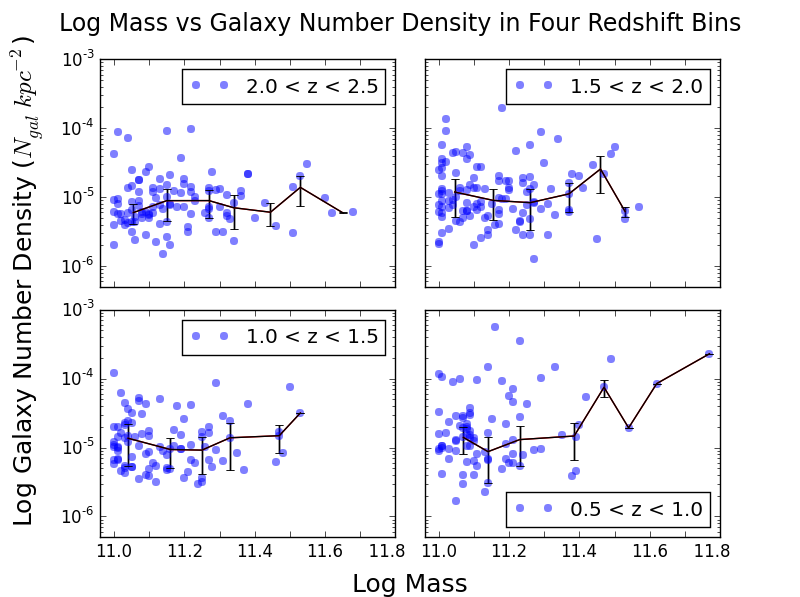
\includegraphics[width=\linewidth]{Mass_Density_Z}
\DeclareGraphicsExtensions{.png}
\caption{\footnotesize All of the galaxies sorted into four bins based on redshift and plotted with mass versus local galaxy number density (both on logarithmic scales). The black line represents the median point of eight mass bins for each subplot. There are error bars for the median absolute deviation of each median point. There is less variation of galaxy density with higher redshifts.}
\label{fig:nth}
\end{figure}

More stuff happens as Mass increases. lets talk about it. See figure~\ref{fig:nth}

PUT IN APERTURE RADIUS MASS GRAPHIC

\section{Summary}

lots and lots and lots and lots andlots and lots andlots and lots andlots and lots andlots and lots andlots and lots andlots and lots andlots and lots andlots and lots andlots and lots andlots and lots andlots and lots andlots and lots andlots and lots andlots and lots andlots and lots andlots and lots andlots and lots andlots and lots andlots and lots andlots of text.


\acknowledgements

\appendix

\begin{thebibliography}{9}

\bibliographystyle{plainnat}

\bibitem{TOMER} Tomer Tal, 2012.

\end{thebibliography}


\end{document}
